%Chapter "Periodic media"
%
\chapter{Periodic media problems}

A periodic material is defined as the repetition of a given motif in one, two or three dimensions. This motif refers to heterogeneities at micro-structural level and it can contains several materials and diverse geometries. These materials can be solids or fluids.

A periodic material is completely described by a lattice and a elementary unit, that is termed \emph{elementary cell}. The lattice is defined by a vector base, and the dimension of thi base is the number of direction for the periodicity.  This set is called lattice \emph{base vectors}, and they allow to build the whole material applying successive translation operations \cite{book:brillouin2003}. For periodic material in 3D, we will denote the base vectors as $\mathbf{a}_1$, $\mathbf{a}_2$ and $\mathbf{a}_3$ (see Figure \ref{fig:periodic_3D}). In the case of 2D periodicity, we can have a material that is infinite or finite in the third dimension (see Figure \ref{fig:periodic_2D}), we denote the vectors as $\mathbf{a}_1$ and $\mathbf{a}_2$. There is also possible to have periodic materials in one direction, and this one can be finite or infinite in the other two directions.

The mesh generator \texttt{gmsh} provides an option to link elements in opposite sides.
\cite{gmsh_manual}. Finite Element Method Magnetic (FEMMM) provides the option of \emph{periodic} boundary conditions, where Multipoint constraints are imposed, this are used for approximation of infinite boundary conditions \cite{FEMM_manual}.

\begin{figure}[h]
\centering
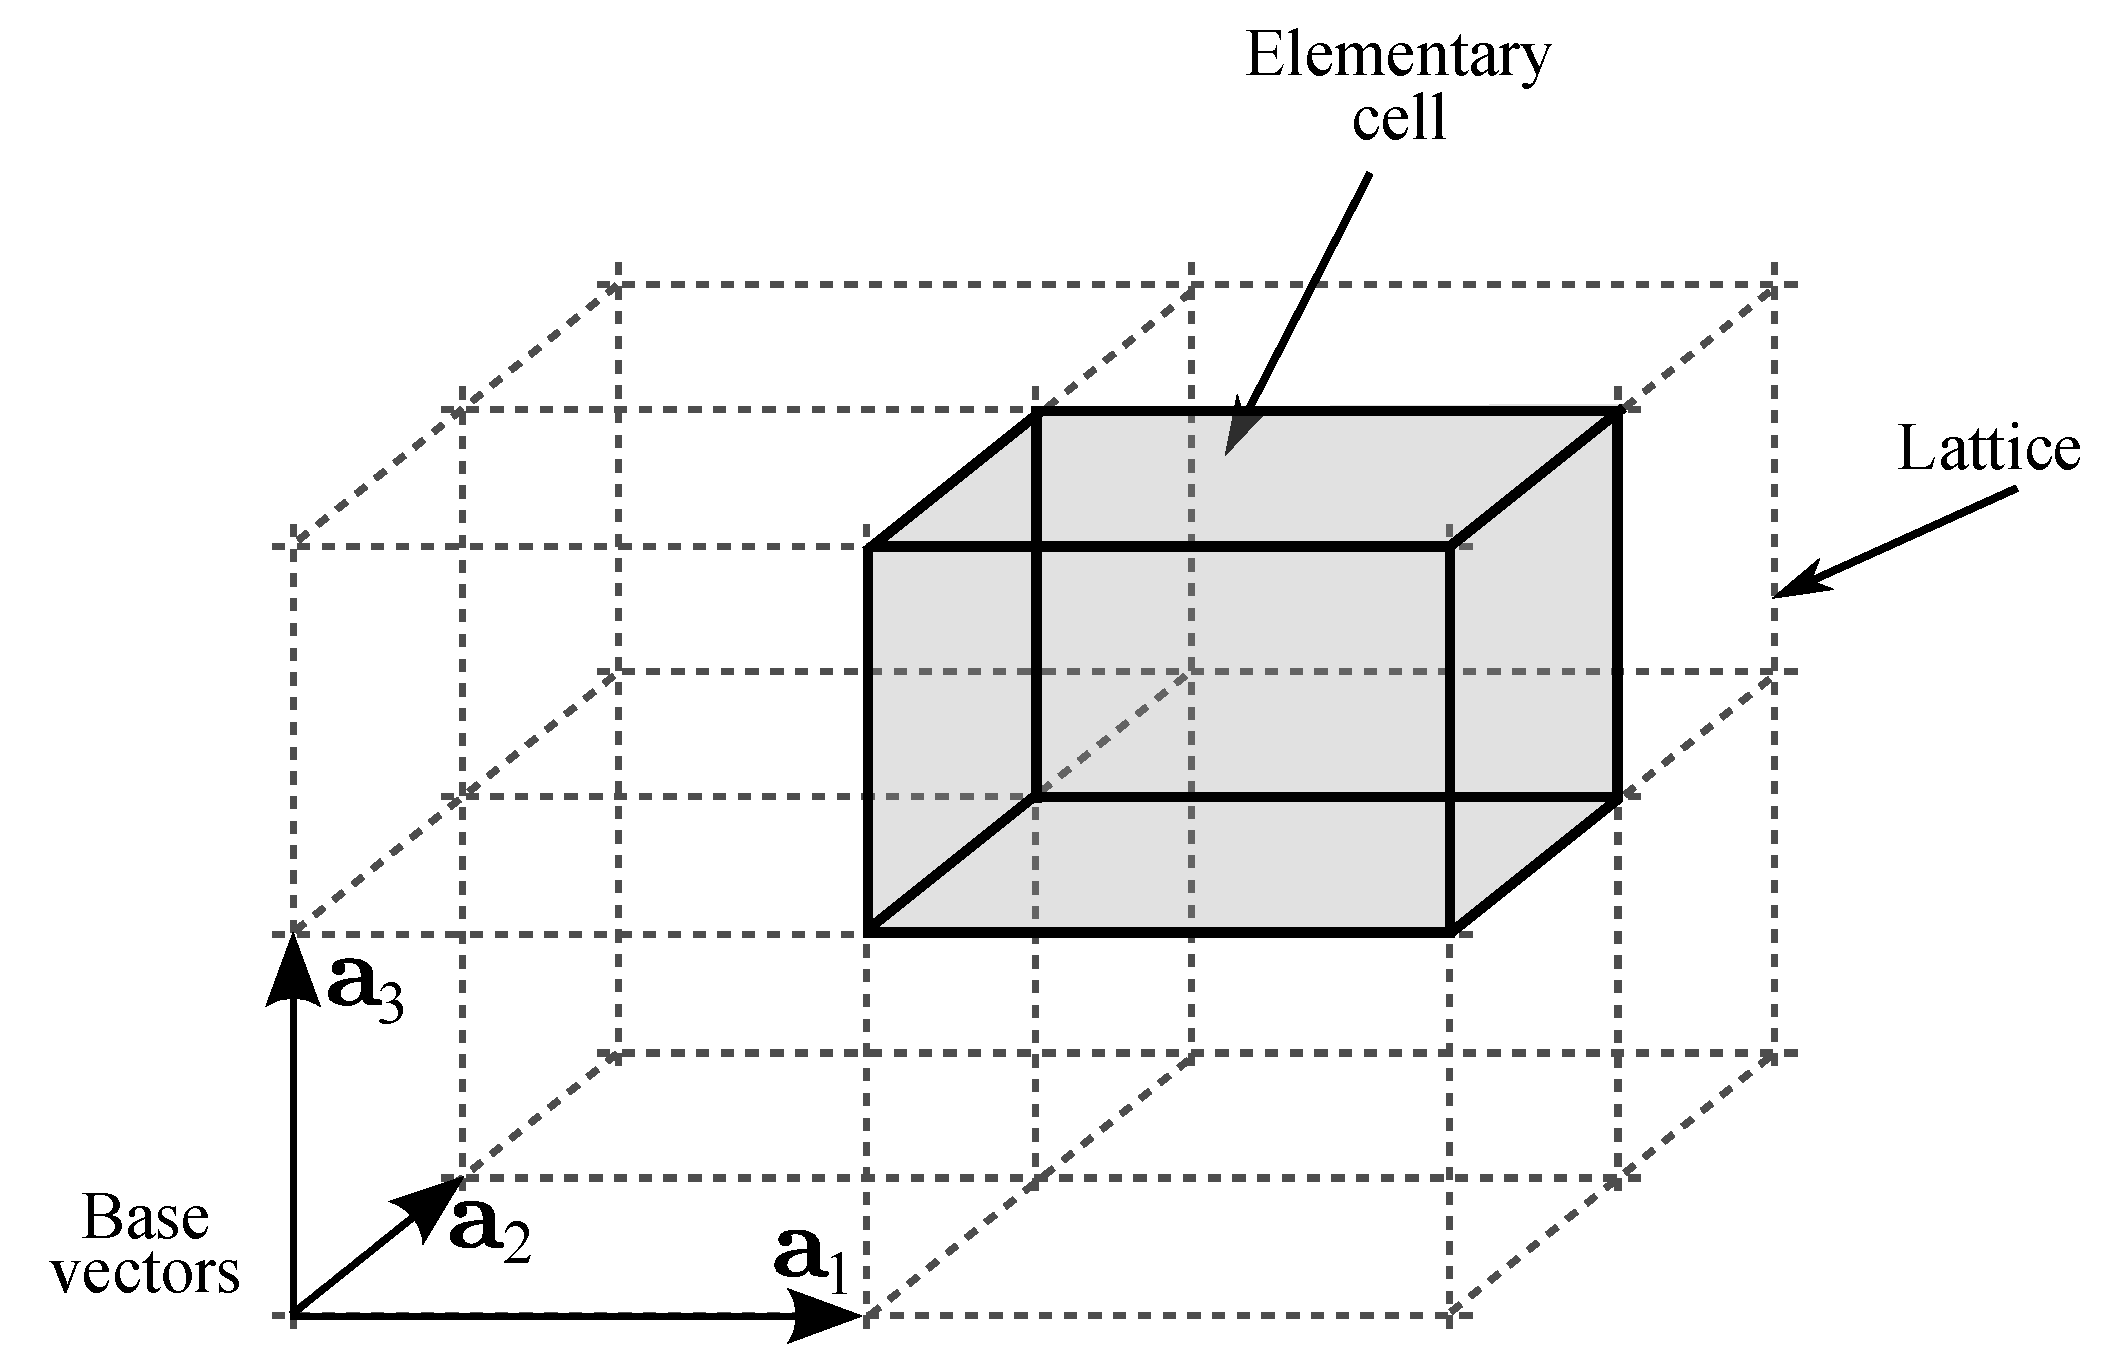
\includegraphics[height=8cm]{img/periodic_3D.pdf} 
\caption{Depiction of a periodic material in 3D.}
\label{fig:periodic_3D}
\end{figure}

\begin{figure}[h]
\centering
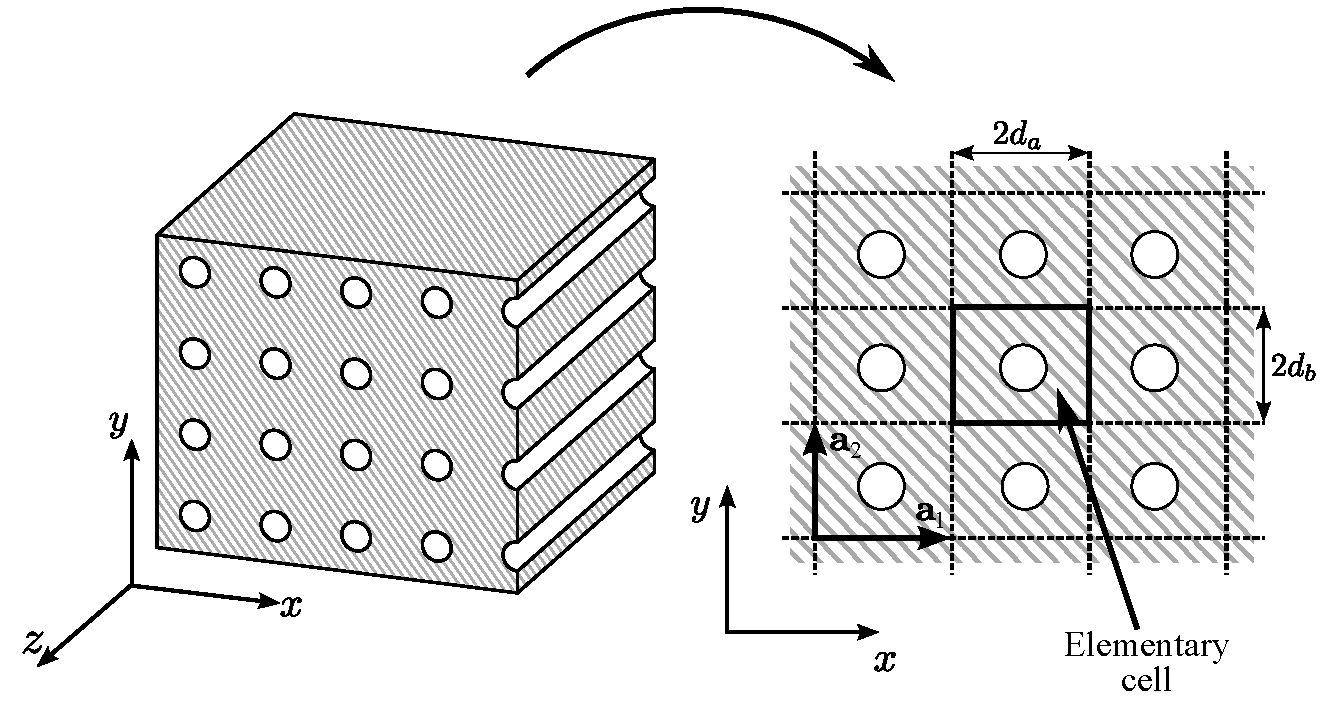
\includegraphics[height=8cm]{img/periodic_2D.pdf} 
\caption{Depiction of a periodic material in 2D.}
\label{fig:periodic_2D}
\end{figure}

\todo{Add Periodic media info.} Describe periodic boundary conditions and Bloch theorem as boundary conditions.

\begin{figure}[h]
\centering
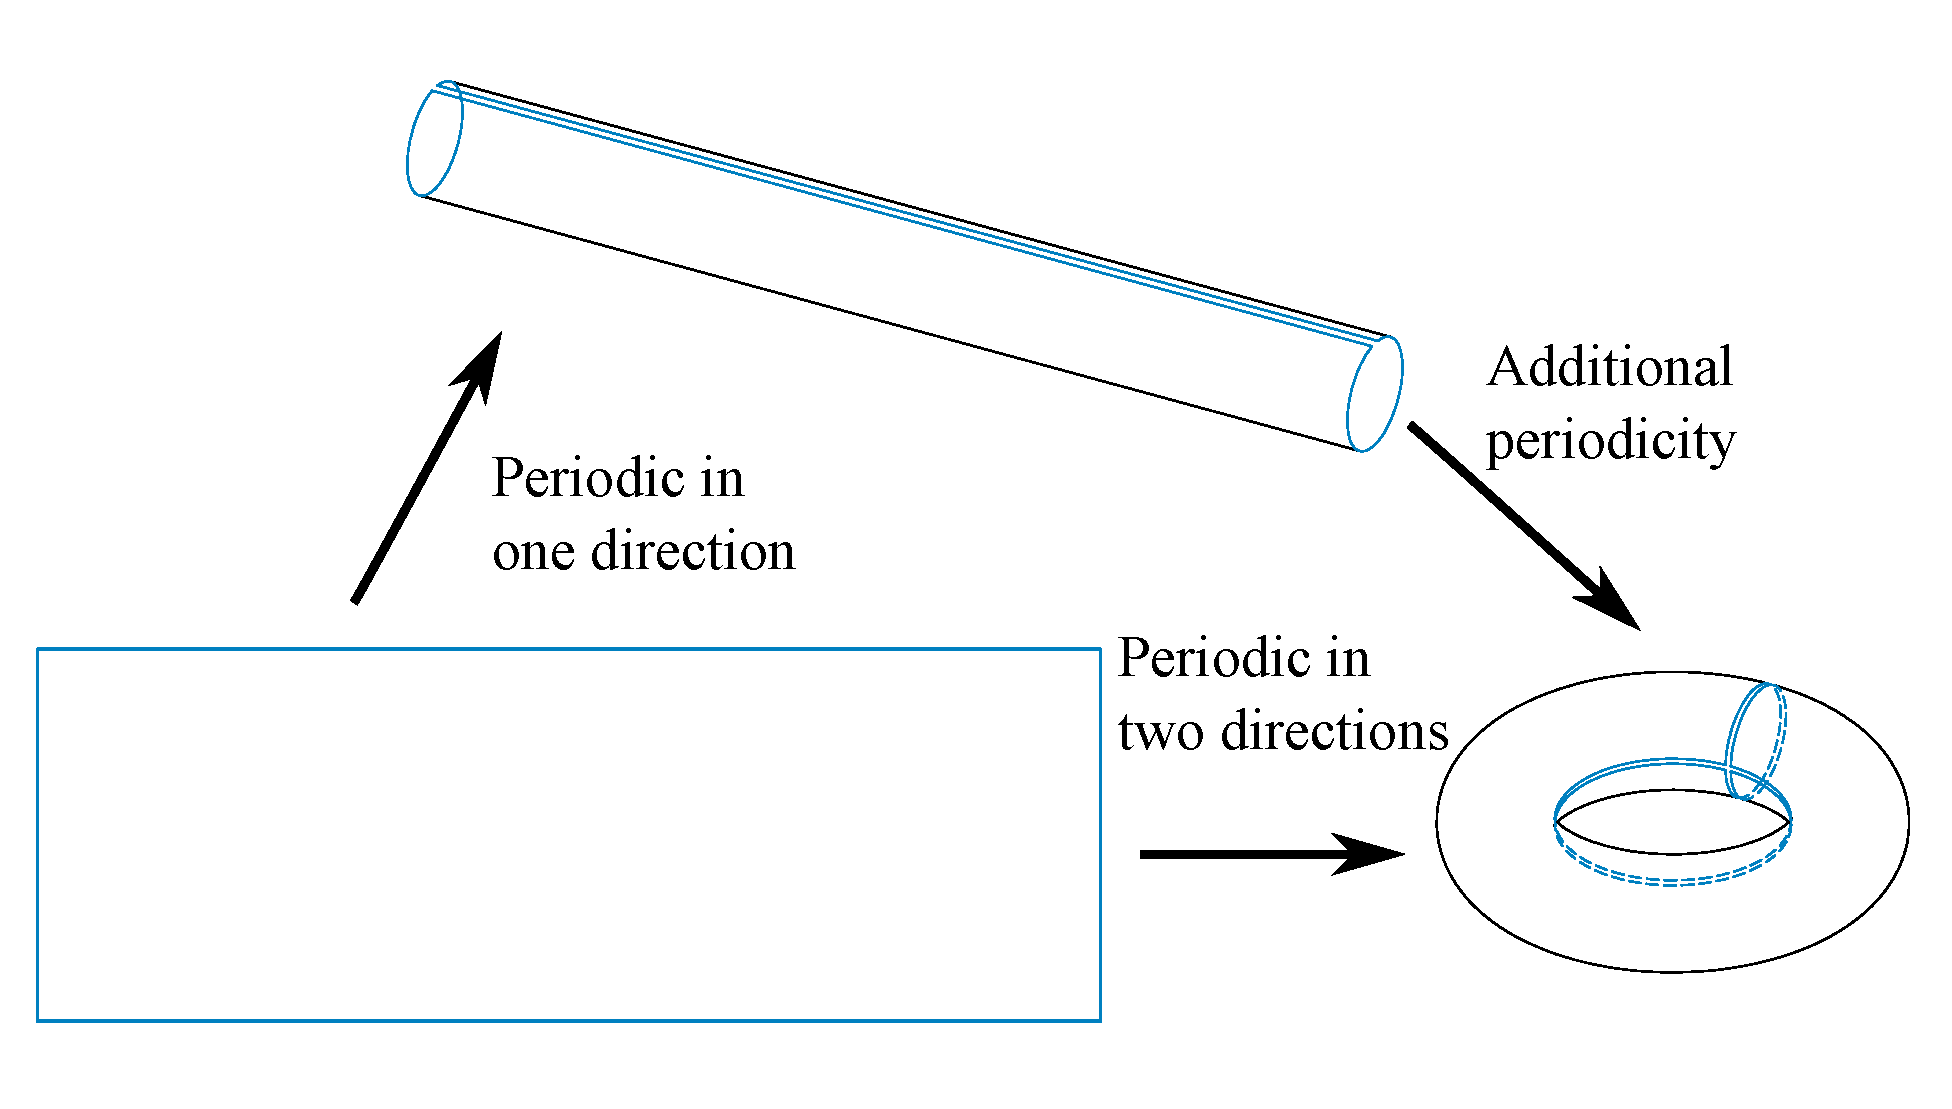
\includegraphics[height=9cm]{img/periodic_topology.pdf} 
\caption{Topology for a rectangular region with periodic boundary conditions.}
\label{fig:periodic_topo}
\end{figure}

Periodic boundary conditions are common in molecular dynamics and micromechanics/homogenization.

\section{Bloch theorem}
Let us start from an equation of the form
\begin{equation}
 Lu(\mathbf{x}) = \omega^2 u(\mathbf{x}) \enspace ,
\label{eq:operator_eigenvalues}
\end{equation}
where $L$ is a differential operator with algebraic properties that are similar to the wave equation \cite{algebraic_waves}. The Bloch theorem establishes that the solution for  \eqref{eq:operator_eigenvalues} is given by
%
\begin{equation}
 u(\mathbf{x}) = w(\mathbf{x}) e^{i\mathbf{k}\cdot\mathbf{x}} \enspace ,
\label{eq:bloch_theorem}
\end{equation}
%
where $w(\mathbf{x})$ is function with the same periodicity of the material and is termed Bloch function. The theorem according to \cite{book:kittel1986} states
%
\begin{quote}
\emph{The eigenfunctions of the wave equation for a periodic potential are the product of a plane wave $\exp(i\mathbf{k}\cdot\mathbf{r})$ times a function $u_\mathbf{k}(\mathbf{r})$ with the periodicity of the crystal lattice.}
\end{quote}
%
If we write the solution \eqref{eq:bloch_theorem} for the point $\mathbf{x}+\mathbf{a}$, we obtain
\[
u(\mathbf{x} + \mathbf{a}) = w(\mathbf{x} + \mathbf{a}) e^{i\mathbf{k}\cdot(\mathbf{x} + \mathbf{a})} \enspace ,
\]
being $\mathbf{a} = n_i \mathbf{a}_i$ a vector with the periodicity of the lattice, and  $n_i \in \mathbb{Z}$. Since$w(\mathbf{x})$ should present the same periodicity of the lattice
\[
u(\mathbf{x} + \mathbf{a}) = w(\mathbf{x}) e^{i\mathbf{k}\cdot(\mathbf{x} + \mathbf{a})} \enspace ,
\]
implying
\[
w(\mathbf{x}) = u(\mathbf{x}+ \mathbf{a}) e^{-i\mathbf{k}\cdot(\mathbf{x} + \mathbf{a})} \enspace ,
\]
and substituting this in \eqref{eq:bloch_theorem}, we get
\begin{equation}
u(\mathbf{x} + \mathbf{a}) = u(\mathbf{x}) e^{i\mathbf{k}\cdot\mathbf{a}} \enspace .
\label{eq:bloch_theorem2}
\end{equation}
Equation \eqref{eq:bloch_theorem2} is termed Bloch periodicity or Bloch-periodic condition. Besides the form in equation \eqref{eq:operator_eigenvalues}, we can also have an equation of the form
\begin{equation}
 Lu(\mathbf{x}) = \omega^2 u(\mathbf{x})  + \mathbf{f}(\omega) \enspace ,
\end{equation}
where $\mathbf{f}(\omega)$ is a harmonic body force with circular frequency $\omega$ that presents the same periodicity that the lattice, see \cite{langlet-thesis}.

\subsection{Bloch theorem in elastodynamics}
Let us consider the wave propagation in an elastic, linear isotropic material. This is described using the Navier-Cauchy equation in the frequency domain (neglecting body forces)
\[ (\lambda + \mu)\nabla(\nabla\cdot \mathbf{u}) + \mu \nabla\times(\nabla\times\mathbf{u})= -\omega^2\rho\mathbf{u} \enspace . \]
The displacement vector can be expressed as $\mathbf{u}=\nabla\varphi + \nabla\times \boldsymbol{\psi}$ due to Helmholtz decomposition theorem \cite{book:arfken, book:sepulveda_fismat}, and the potentials $\varphi,  \boldsymbol{\psi}$ are the scalar and vector potential, respectively. These potential verify
\begin{align*}
\nabla^2\varphi = -\frac{\omega^2}{\alpha^2} \varphi \enspace , \\
\nabla^2 \boldsymbol{\psi} = -\frac{\omega^2}{\beta^2} \boldsymbol{\psi} \enspace ,
\end{align*}
where $\alpha, \beta$ correspond with the speed for the longitudinal and transverse waves.

Since the equations for the potentials $\varphi,  \boldsymbol{\psi}$ are wave equations, they satisfy Bloch theorem and then
\begin{align*}
\varphi(\mathbf{x}) = \varphi(\mathbf{x}+\mathbf{a})e^{i\mathbf{k}\cdot \mathbf{a}} ,\\
 \boldsymbol{\psi}(\mathbf{x}) =  \boldsymbol{\psi}(\mathbf{x}+\mathbf{a})e^{i\mathbf{k}\cdot \mathbf{a}} \enspace ,
\end{align*}
and
\begin{align*}
\mathbf{u}(\mathbf{x}) &= \nabla\varphi(\mathbf{x}) + \nabla\times \boldsymbol{\psi}(\mathbf{x}) = e^{i\mathbf{k}\cdot\mathbf{a}}\nabla\varphi(\mathbf{x}) + e^{i\mathbf{k}\cdot\mathbf{a}}\nabla\times \boldsymbol{\psi}(\mathbf{x}) ,\\
&= e^{i\mathbf{k}\cdot\mathbf{a}}\left[ \nabla\varphi(\mathbf{x}) + \nabla\times \boldsymbol{\psi}(\mathbf{x}) \right] =  e^{i\mathbf{k}\cdot\mathbf{a}}\mathbf{u}(\mathbf{x}+\mathbf{a}) \enspace .
\end{align*}
Thus, the Bloch theorem is satisfied for the displacement field, i.e.
\[\mathbf{u}(\mathbf{x}) = e^{i\mathbf{k}\cdot\mathbf{a}} \mathbf{u}(\mathbf{x}+\mathbf{a}) \enspace .\]

\section{Bloch theorem as boundary conditions}
If we start from the reduced wave equation \cite{book:achenbach_waves} the boundary value problem would be given by
\begin{align*}
&(\lambda +2\mu)\nabla(\nabla\cdot \mathbf{u}) + \mu \nabla\times(\nabla\times\mathbf{u})= -\omega^2\rho\mathbf{u}  &\text{in\ } \Omega,\\
&\mathbf{u}(\mathbf{x}+\mathbf{a}) = \mathbf{u}(\mathbf{x})e^{i\mathbf{k}\cdot\mathbf{a}} &\text{in\ } \Gamma_u,\\
&\mathbf{t}(\mathbf{x}+\mathbf{a}) = -\mathbf{t}(\mathbf{x})e^{i\mathbf{k}\cdot\mathbf{a}} &\text{in\ } \Gamma_t \enspace .
\end{align*}
We will call this type of boundary conditions \emph{Bloch-periodicity}\footnote{Periodic boundary conditions are a particular case, where the factor $e^{i\mathbf{k}\cdot\mathbf{a}}=1$.}. The operator of this partial differential equation is self-adjoint and positive definite for Bloch-periodic conditions \cite{book:reddy_functional_analysis, book:kreyzsig_functional}, thus the eigenvalues are real and positive. After discretization (using FEM), the resulting matrices are Hermitian and positive definite. What makes sense from a physical point of view, the energy of the system is always bigger than zero and the eigenvalues (squared frequencies) must be positive.

The problem can be equivalently formulated for the Bloch function $\mathbf{w}(\mathbf{x})$, where the Bloch-periodic conditions are replace by (plane) periodic conditions \cite{book:PDE_gockenbach}. The equivalent boundary value problem is
\begin{align*}
&B\mathbf{w} = -\omega^2\rho\mathbf{w} &\text{in\ } \Omega,\\
&\mathbf{w}(\mathbf{x}+\mathbf{a}) = \mathbf{w}(\mathbf{x}) &\text{in\ } \Gamma_u,\\
&\frac{\partial \mathbf{w}}{\partial \hat{\mathbf{n}} }(\mathbf{x}+\mathbf{a}) = \frac{\partial \mathbf{w}}{ \partial \hat{\mathbf{n}} }(\mathbf{x}) &\text{in\ } \Gamma_t \enspace ,
\end{align*}
where $B$ is the operator
\[B = (\lambda+\mu)\left[ \nabla\nabla\cdot + i\lbrace\mathbf{k}\nabla\cdot + \mathbf{k}\cdot\nabla + \mathbf{k}\times\nabla\times\rbrace\right]() - \mu\left[ \nabla^2 + 2i\mathbf{k}\cdot\nabla - \Vert \mathbf{k} \Vert^2 \right]() \enspace .\]

\section{Variational form for elastodynamics with Bloch-periodicity}
Let us start from the momentum equation in the frequency domain
\[\sigma_{rs,s}+f_{r}(\omega) = -\rho \omega^2 u_r,\ \text{en } \Omega,\]
where $f_r$ is a harmonic force in the direction $r$, $\sigma_{rs}=C_{rskl}\epsilon_{kl}$ and $\epsilon_{kl} =1/2(u_{k,l} + u_{l,k})$. The boundary conditions are
\begin{subequations}
\begin{align}
u_r(x_s +a_s)=u_r(x_s)e^{i k_s a_s}\ \text{in } \Gamma_u, \label{eq:disp_bloch}\\
t_r(x_s +a_s)=-t_r(x_s)e^{i k_s a_s}\ \text{in } \Gamma_t, \label{eq:force_bloch}
\end{align}
\label{eq:bloch_cond}
\end{subequations}
being $t_{r}$ the traction on the surface of the cell.

Now, let us multiply the momentum equation by the complex conjugate of an arbitrary function $v_r$ and integrate over the domain\footnote{In the deduction of weak forms for FEM it is customary to multiply by a function $v_r$ that is real. In this case the function is complex; in order to satisfy the properties for an inner product, we need to multiply by the complex conjugate (see for example  \cite{sukumar_bloch-2009, book:arfken}).}
\[\int\limits_{\Omega} v_r^{*}[\sigma_{rs,s} + f_r(\omega)]d \Omega = -\omega^2 \int\limits_{\Omega} \rho v_r^{*} u_r d \Omega \enspace , \]
the complex conjugate is denoted by $*$. Then, using the constitutive relation
\[\int\limits_{\Omega} v_r^{*}C_{rskl}\epsilon_{kl,s}d \Omega + \int\limits_{\Omega} v_r^{*}f_r d \Omega = -\omega^2 \int\limits_{\Omega} \rho v_r^{*} u_r d \Omega \enspace , \]
and using divergence theorem
\[-\int\limits_{\Omega} v_r,s^{*}C_{rskl}\epsilon_{kl}d \Omega + \int\limits_{\Omega}v_r^{*}t_r(n_s)d \Gamma +  \int\limits_{\Omega} v_r^{*}f_r d \Omega = -\omega^2 \int\limits_{\Omega} \rho v_r^{*} u_r d \Omega \enspace , \]
with $t_r^{n_s} = C_{rskl}\epsilon_{kl}n_{s}$, if we take $v_r = u_r$ and consider that the tensor $\epsilon_{rs}$ is symmetric, we obtain
\[ -\int\limits_{\Omega} \epsilon_{rs}C_{rskl}\epsilon_{kl} d \Omega + \int\limits_\Gamma u_r^{*} t_{r}(n_s) d \Gamma \int\limits_\Omega u_r^{*}f_r(\omega) d\Omega = -\omega^2\int\limits_\Omega \rho u_r^{*} u_r d\Omega \enspace . \]
And neglecting the body forces, the Energy Functional for this problem is written as
\begin{equation}
\Pi(\omega) = \int\limits_\Omega \epsilon_{rs}^{*}(\mathbf{x})C_{rskl}(\mathbf{x})\epsilon_{kl}(\mathbf{x}) d \Omega - \omega^2\int\limits_\Omega \rho(\mathbf{x})u_r^{*}(\mathbf{x})u_r(\mathbf{x}) d\Omega - \int\limits_{\Gamma} u_r^{*}(\mathbf{x})t_r(\mathbf{x}) d\Gamma \enspace .
\label{eq:energy_functional}
\end{equation}
The first term in the equation \eqref{eq:energy_functional} is the deformation energy inside the domain, the second term corresponds with the kinetic energy for harmonic motion with angular frequency $\omega$, the last term is the deformation energy on the boundary of the domain. The boundary term is related with the imposition of natural boundary conditions (Neumann BCs) in the formulation of the FEM. In this case the Bloch-periodic conditions for the forces are implicitly satisfied  in the variational form, as we will see in detail.

Since the domain is a single cell of a lattice, it should form a tessellation \footnote{A tessellation is a regular pattern that covers all the space with no overlaps and no gaps.}. Hence, the boundaries can be grouped by pairs, i.e., each side (\emph{reference side}) should have an opposite side  (\emph{image side}), so the last term in \eqref{eq:energy_functional}can be rewritten as
\[ \int\limits_{\Gamma} u_r^{*}(\mathbf{x}) t_r(\mathbf{x}) d\Gamma = \sum\limits_{l} \int\limits_{\Gamma_l} [ u_r^{*}(\mathbf{x}) t_r(\mathbf{x}) + u_r^{*}(\mathbf{x+\mathbf{a}_l}) t_r(\mathbf{x}+\mathbf{a}_l) ]d\Gamma \enspace ,\]
where the index $l$ refers to each one of the pairs of opposite sides in the boundary. Thus
\begin{align*}
\int\limits_{\Gamma} u_r^{*}(\mathbf{x}) t_r(\mathbf{x}) d\Gamma &= \sum\limits_{l} \int\limits_{\Gamma_l} [ u_r^{*}(\mathbf{x}) t_r(\mathbf{x}) +e^{-i\mathbf{k}\cdot\mathbf{a}_l} u_r^{*}(\mathbf{x}) t_r(\mathbf{x}+\mathbf{a}_l) ]d\Gamma \enspace , \\
\int\limits_{\Gamma} u_r^{*}(\mathbf{x}) t_r(\mathbf{x}) d\Gamma &= \sum\limits_{l} \int\limits_{\Gamma_l} u_r^{*}(\mathbf{x})[ t_r(\mathbf{x}) +e^{-i\mathbf{k}\cdot\mathbf{a}_l} t_r(\mathbf{x}+\mathbf{a}_l) ]d\Gamma \enspace ,
\end{align*}
and the expression in square brackets is the condition \eqref{eq:force_bloch}, that is equal to zero. This variational form can be computed for other operators that have similar algebraic properties to wave equations and are positive definite \cite{algebraic_waves, book:reddy_functional_analysis, book:kreyzsig_functional}.

\section{Implementation}
\subsection{Bloch-periodicity in FEM}
The Bloch-periodic conditions in a Finite Element problem or, more generally, in a discrete problem can be formulated as a set of relations between the degrees of freedom of opposite sides of the unit cell.
\begin{figure}[h]
\centering
	\begin{subfigure}[b]{0.3\textwidth}
		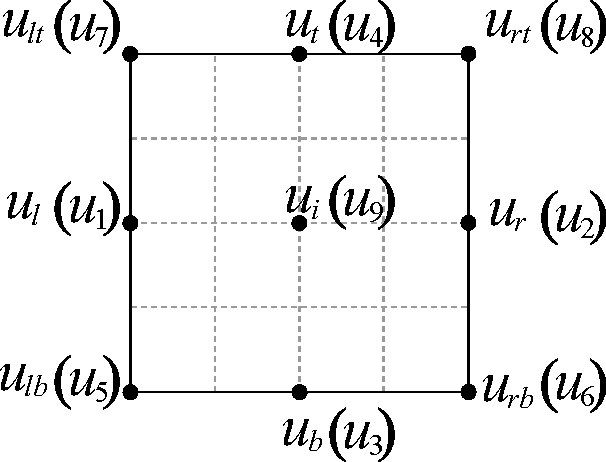
\includegraphics[width=\textwidth]{img/cell_FEM.pdf}
		\caption{Original cell.}
	\end{subfigure}\quad
%
	\begin{subfigure}[b]{0.3\textwidth}\qquad
		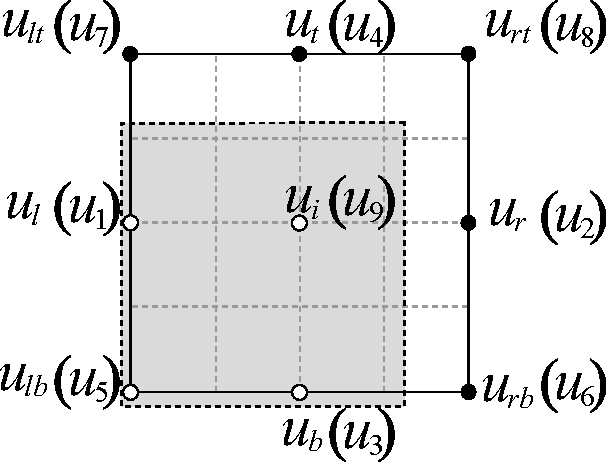
\includegraphics[width=\textwidth]{img/cell_FEM-2.pdf}
		\caption{\emph{Reduced} cell.}
	\end{subfigure}\\
%
	\begin{subfigure}[b]{0.7\textwidth}\qquad
		\centering
		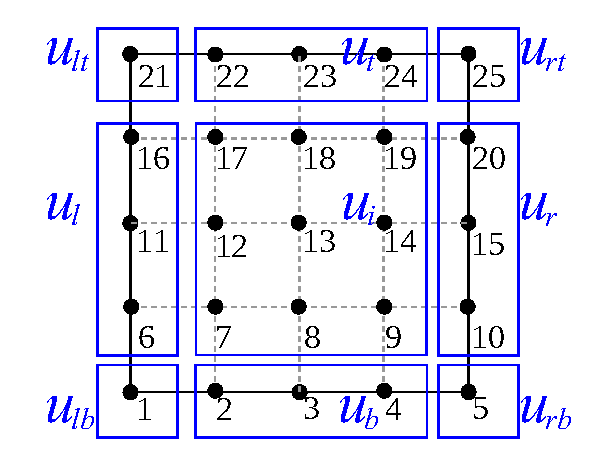
\includegraphics[width=0.45\textwidth]{img/cell_FEM-nodes.pdf}
		\caption{The black circles now correspond to single degrees of freedom. Notice that the nodal numbering does not match the original numbering for groups of degrees of freedom.}
	\end{subfigure}
\caption{Relevant sets of DOF for an schematic unitary cell in 2D discretized with several finite elements. Each circle represents a family of degrees of freedom for a typical mesh and not a single degree of freedom. In part a) we show all the degrees of freedom for the unitary cell before imposing the relevant Bloch-periodic boundary conditions. Part b) shows the reduced cell where the white circles enclosed by the dark square represent the \emph{reference} nodes containing the information from the \emph{image} nodes which will be eventually deleted from the system. Part c) shows an example of node grouping for a mesh of $4\times 4$ elements.}
\label{fig:bloch_FEM}
\end{figure}

In three dimension, and periodicity or Bloch-periodicity in the three of them, we can depict the original and reduced cell in Figure \ref{fig:bloch_3D_cell}. It should be highlighted that in 3D it is possible to have periodicity in 1, 2 or 3 dimensions, depending on the nature of the problem of interest.
\begin{figure}[h]
	\centering
	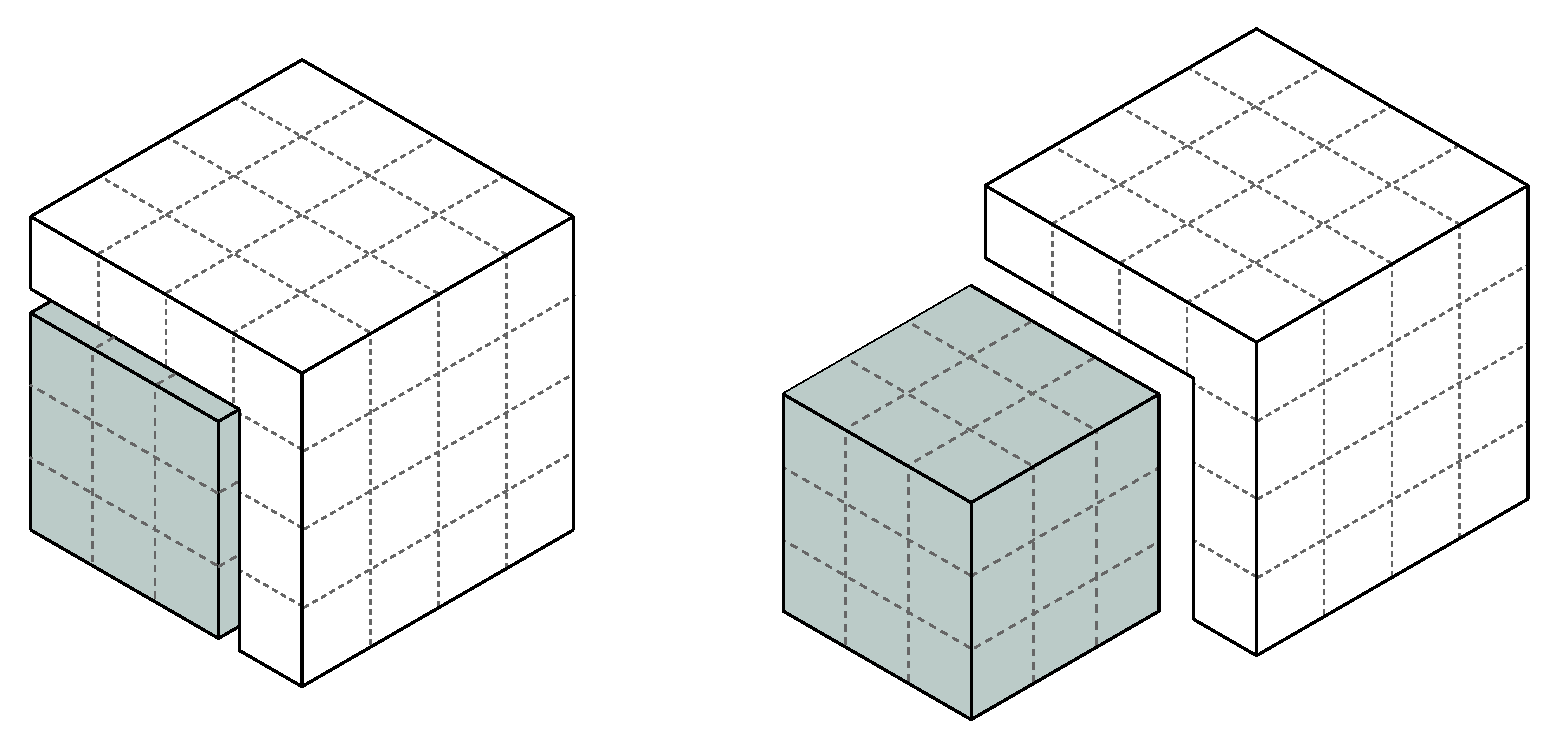
\includegraphics[width=0.65\textwidth]{img/Cube_Bloch_Schematic.pdf}
	\caption{Three dimensional unitary cell with a $4\times4\times4$ mesh. It is partitioned into the image DOF and remaining ones. The reduced cell is highlighted.}
	\label{fig:bloch_3D_cell}
\end{figure}

Let us start from the original problem
\begin{equation}
[K-\omega^2 M]\lbrace u\rbrace = \lbrace f\rbrace \enspace ,
\label{eq:discrete_system}
\end{equation}
where
\begin{align*}
u &= [u_l\ u_r\ u_b\ u_t\ u_{lb}\ u_{rb}\ u_{lt}\ u_{rt}\ u_{i}]^T = [ u_1\ u_2\ u_3\ u_4\ u_5\ u_6\ u_7\ u_8\ u_9]^T\ , \\
f &= [f_l\ f_r\ f_b\ f_t\ f_{lb}\ f_{rb}\ f_{lt}\ f_{rt}\ f_{i}]^T = [ f_1\ f_2\ f_3\ f_4\ f_5\ f_6\ f_7\ f_8\ f_9]^T\ ,
\end{align*}
the subindices are describe in Figure \ref{fig:bloch_FEM}.

From Bloch theorem we know
\begin{align*}
u_2 = e^{i \psi_x}u_1, \quad u_4 = e^{i \psi_y}u_3,\quad u_6 = e^{i \psi_x}u_5, \\
u_7 = e^{i \psi_y}u_5,\quad u_8 = e^{i (\psi_x + \psi_y)}u_5,
\end{align*}
with $\psi_x = 2 k_x d_a $ and $\psi_y = 2 k_y d_b $ phase shifts in $x$ and $y$, and $(k_x,k_y)=\mathbf{k}$ wave vector. If we think about this relations as a linear transformation we can write
\begin{equation}
\underbrace{\left\lbrace  \begin{array}{c}
u_1 \\ 
u_2 \\ 
u_3 \\ 
u_4 \\ 
u_5 \\ 
u_6 \\ 
u_7 \\ 
u_8 \\ 
u_9
\end{array}  \right\rbrace }_{u} = 
\underbrace{\left[ \begin{array}{cccc}
I_{nl} & 0 & 0 & 0 \\ 
I_{nl} e^{i\psi_x} & 0 & 0 & 0 \\ 
0 & I_{nb} & 0 & 0 \\ 
0 & I_{nb} e^{i\psi_y} & 0 & 0 \\ 
0 & 0 & I_2 & 0 \\ 
0 & 0 & I_2 e^{i\psi_x} & 0 \\ 
0 & 0 & I_2 e^{i\psi_y} & 0 \\ 
0 & 0 & I_2 e^{i(\psi_x + \psi_y)} & 0 \\ 
0 & 0 & 0 & I_{ni}
\end{array} \right] }_{T}
\underbrace{\left\lbrace \begin{array}{c}
u_1 \\ 
u_3 \\ 
u_5 \\ 
u_9
\end{array} 
\right\rbrace }_{u_R} \enspace ,
\label{eq:disp_transformation}
\end{equation}
being $I_{n}$ identity matrices of size $n$ (equal to the number of degrees of freedom associated to each group). We can write the equation \eqref{eq:disp_transformation} in compact form as $u = Tu_R$, and substituting \eqref{eq:disp_transformation} in \eqref{eq:discrete_system} we obtain
\begin{equation}
[KT]{u_R} = \omega^2[MT]{u_R} \enspace .
\label{eq:aux_system}
\end{equation}
Also, from the Bloch theorem we have the following equilibrium conditions
\begin{align*}
f_2 + e^{i \psi_x}f_1=0, \quad f_4 + e^{i \psi_y}f_3=0 , \\
f_8 + e^{i \psi_x}f_6 + e^{i \psi_y}f_7 +e^{i (\psi_x + \psi_y)}f_5 = 0 \enspace .
\end{align*}
And, again, thinking this relations as another linear transformation
\begin{equation}
\underbrace{\left\lbrace  \begin{array}{c}
0 \\ 
0 \\ 
0 \\ 
f_9 
\end{array}  \right\rbrace }_{f_R} = 
\underbrace{\left[ \begin{array}{ccccccccc}
I_{nl} & I_{nl} e^{-i\psi_x} & 0 & 0 & 0 & 0 & 0 & 0 & 0 \\ 
0 & 0 & I_{nb} & I_{nb} e^{-i\psi_y} & 0 & 0 & 0 & 0 & 0 \\ 
0 & 0 & 0 & 0 & I_{2} & I_{2} e^{-i\psi_x} & I_{2} e^{-i\psi_y} & I_{2} e^{-i(\psi_x+\psi_y)} & 0 \\ 
0 & 0 & 0 & 0 & 0 & 0 & 0 & 0 & I_{ni} 
\end{array}  \right] }_{T^H}
\underbrace{\left\lbrace \begin{array}{c}
f_1 \\ 
f_2 \\ 
f_3 \\ 
f_4 \\ 
f_5 \\ 
f_6 \\ 
f_7 \\ 
f_8 \\ 
f_9
\end{array} 
\right\rbrace }_{f} \enspace .
\label{eq:force_transformation}
\end{equation}
Now, we multiply \eqref{eq:aux_system} by $T^H$, where $T^H$ is the Hermitian transpose of $T$,
\begin{equation}
\left[\underbrace{T^HKT}_{K_R} - \omega^2\underbrace{T^HKT}_{M_R} \right] \lbrace u_R\rbrace = \lbrace f_R\rbrace \enspace .
\label{eq:transfo_bloch}
\end{equation}
The new system of equations is of size $n\times n$, being $n$ the number of independent variables in  $u_R$, and the matrices  $K_R$, $M_R$ are Hermitian. This conditions is derived from the fact that the original matrices $K$, $M$ are real and symmetric. Neglecting the body forces $f_R$ we obtain the generalized eigenvalue problem for the reduced system
\begin{equation}
[K_R]\lbrace u_R\rbrace = \omega^2 [M_R] \lbrace u_R\rbrace \enspace .
\end{equation}

The implementation of the periodic and Bloch-periodic boundary conditions can be achieved in two different ways:
\begin{itemize}
\item changing the connectivity, and the respective interpolation functions (see Figure \ref{fig:bloch_interp}); or
\item assembling the mass and stiffness matrices assuming they do not have boundary conditions and then, using elementary row operations and elementary column operations, obtain the matrices with the desired conditions.
\end{itemize}
The modification over the mesh is well illustrated in Figure \ref{fig:bloch_interp}, where the continuity is warranted in the periodic case and a phase shift appears for the Bloch-periodic one.
\begin{figure}[H]
\centering
	\begin{subfigure}[b]{0.4\textwidth}\qquad
		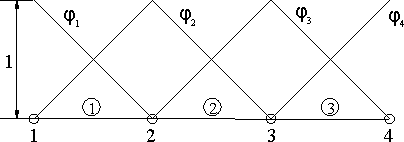
\includegraphics[width=\textwidth]{img/periodic-interpolation-a.pdf}
		\caption{Neumann conditions. }
	\end{subfigure}\,
%
	\begin{subfigure}[b]{0.4\textwidth}\qquad
		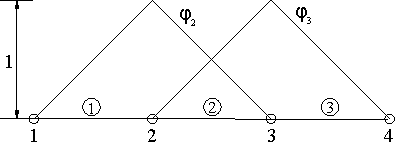
\includegraphics[width=\textwidth]{img/periodic-interpolation-b.pdf}
		\caption{Dirichlet conditions.}
	\end{subfigure}\\
%
	\begin{subfigure}[b]{0.4\textwidth}\qquad
		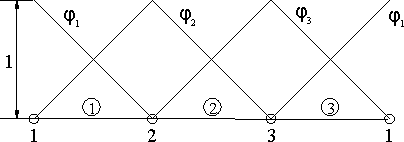
\includegraphics[width=\textwidth]{img/periodic-interpolation-c.pdf}
		\caption{Periodicity conditions.}
	\end{subfigure}\,
%
	\begin{subfigure}[b]{0.4\textwidth}\qquad
		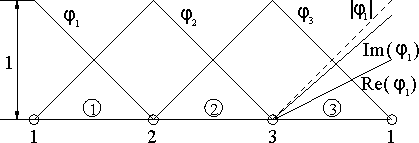
\includegraphics[width=\textwidth]{img/periodic-interpolation-d.pdf}
		\caption{Bloch-periodicity conditions.}
	\end{subfigure}
\caption{Basis functions for linear finite elements.
 (a) Neumann conditions; (b) Dirichlet conditions; (c) Periodic conditions; and (d) Bloch-periodic conditions. The real and imaginary part of $\varphi_1$ are illustrated in the basis with Bloch conditions in (d) for a phase shifts of $ka=\pi/3 (\omega=[0,a])$. The modulus of $\varphi_1$ is the same at $x=0$ and at $x=a$.}
\label{fig:bloch_interp}
\end{figure}
When obtaining the matrices without boundary conditions, the \emph{reduced} matrices can be obtained in two different ways. One of them is applying elementary operations. We call the nodes of one side  \emph{reference nodes} and the corresponding opposite nodes \emph{image nodes}. The procedure to obtain the reduced matrices is \cite{sukumar_bloch-2009, MSc_thesis-Guarin2012}
\begin{itemize}
\item Multiply the elements of $A_{kl}$ associated with a boundary node by $f_k^{*}f_l$.
\item For each row $i$ of $A$ associated with a reference node, add all the rows $k$ associated with the corresponding image nodes. For each column $j$ associated with a reference node, add all the columns $l$ associated with the corresponding image nodes.
\item Eliminate all the rows $k$ and columns $l$ associates with image nodes.
\end{itemize}
The factor $f_j=e^{i\mathbf{k}\cdot \mathbf{x}_j}$, where $\mathbf{x}_j$ are the coordinates of the $j$th node and $f^{*}$ is the complex conjugate of $f$. A complete  description is presented in \cref{algo:bloch_op}.

\begin{algorithm}[h] 
\DontPrintSemicolon
\SetKwInOut{Input}{Input}\SetKwInOut{Output}{Output}
\Input{	A: Original matrix \\
		$k_x$, $k_y$: wave-vector components\\
		nodes: array with nodal coordinates\\
		image, reference: array with corresponding image and reference nodes\\
		reference2: array with reference nodes without repetition\\
}
\Output{Matrix A with imposed Bloch's conditions}
\BlankLine
\For(\tcp{Phase shift for image nodes}){ i=1 \KwTo n\_img}{
   img\_index $\leftarrow$ image[i]\;
   x\_img $\leftarrow$ nodes[img\_index,1]\;
   y\_img $\leftarrow$ nodes[img\_index,2]\;
   fac $\leftarrow e^{i k_x \text{x\_img}}e^{i k_y \text{y\_img}}$\;
   A[img\_index, :] $\leftarrow$ A[img\_index, :]fac\;
   A[:, img\_index] $\leftarrow$ A[:, img\_index]fac$^{*}$\;
}
\For(\tcp{Phase shift for reference nodes}){ i=1 \KwTo n\_ref}{
   ref\_index $\leftarrow$ reference2[i]\;
   x\_ref $\leftarrow$ nodes[ref\_index,1]\;
   y\_ref $\leftarrow$ nodes[ref\_index,2]\;
   fac $\leftarrow e^{i k_x \text{x\_ref}}e^{i k_y \text{y\_ref}}$\;
   A[ref\_index, :] $\leftarrow$ A[ref\_index, :]fac\;
   A[:, ref\_index] $\leftarrow$ A[:, ref\_index]fac$^{*}$\;
}
\For(\tcp{Addition of image row/columns to reference row/colums}){ i=1 \KwTo n\_cond}{
   img\_index $\leftarrow$ image[i]\;
   ref\_index $\leftarrow$ reference[i]\;
   A[ref\_index, :] $\leftarrow$ A[ref\_index, :] + A[img\_index, :]\;
   A[:, ref\_index] $\leftarrow$ A[:, ref\_index] + A[:,img\_index, :]\;
}
\For(\tcp{Elimination of image row/columns}){ i=1 \KwTo n\_imag}{
   img\_index $\leftarrow$ image[i]\;
   A[img\_index, :] $\leftarrow$ erase row img\_index from A\;
   A[img\_index, :] $\leftarrow$ erase column img\_index from A\;
}
\caption{Imposition of Bloch's conditions using elemental row operations.}\label{algo:bloch_op}
\end{algorithm}

Another way to impose the Bloch-periodic conditions is to \emph{assemble} the transformation matrix $T$ and compute the matrix multiplications shown in \eqref{eq:transfo_bloch}. After applying this procedure the \emph{image nodes} are removed from the system of equations and they are condensed in the correspondid reference nodes \cite{langlet-thesis, hladky-hennion1992}, and the equation identifiers (equations enumeratino) have changed. The procedure to assemble the matrix $T$ is:
\begin{itemize}
\item Find the new identifier for the reference nodes after eliminating the image nodes.
\item For reference and interior nodes correspond a 1 in the matrix. The row is the current identifier and the column is the future one.
\item For image nodes correspond the complex number $e^{ik_x (x_\text{img}-x_\text{ref})}e^{ik_y (y_\text{img}-y_\text{ref})}$ in the matrix; being $x_\text{ref},x_\text{img},y_\text{ref},y_{img}$ the coordinates $x,y$ for the reference an image nodes. The row is the identifier for that image node and the column is the future identifier for the corresponding reference node.
\item The remaining entries of the matrix are zeros.
\end{itemize}
This procedure is equivalent to arrange the elementary row/column operations for the procedure described above in a matrix \cite{algebra_lineal-poole}. This procedure is described with further insight in Algorithm \ref{algo:bloch_matrix}.
\begin{algorithm}[h]  
\DontPrintSemicolon
\SetKwInOut{Input}{Input}\SetKwInOut{Output}{Output}
\Input{	A: Original matrix \\
		$k_x$, $k_y$: wave-vector components\\
		nodes: array with nodal coordinates\\
		image, reference: array with corresponding image and reference nodes\\
		reference2: array with reference nodes without repetition\\
}
\Output{Matrix A with imposed Bloch's conditions}
\BlankLine
index\_vec $\leftarrow \vec{0}$   \tcp{Array with new equation identifiers}
\For(){ i=1 \KwTo ncond}{
	index\_vec[image[i]] $\leftarrow$ - reference[i] \tcp{Negative of the current identifier for the reference node}
}
\For(\tcp{Assign new identifiers}){ i=1 \KwTo ndof}{
	cont $\leftarrow$ 0\;
	\For(\tcp{How many image nodes before the current one}){ j=1 \KwTo ncond}{
		\uIf{$index\_vec[i]<0$}{
			\If(){$image[j]< | index\_vec[i]|$}{
				cont $\leftarrow$ cont + 1 \;
			}
		}
		\ElseIf{$image[j]<i$}{
			cont $\leftarrow$ cont + 1\;	
		}
	}
	\eIf(\tcp{Assign new identifiers}){$index\_vec[i]<0$}{
		index\_vec[i] $\leftarrow$ index\_vec[i] + cont\;		
	}{
		index\_vec[i] $\leftarrow$ i - cont\;	
	}
}
T $\leftarrow 0$;\qquad index\_ref $\leftarrow$ - index\_vec\;
\For(){i=1 \KwTo ndof}{
	\eIf{ $index\_vec[i] > 0$}{
		j $\leftarrow$ index\_vec[i]\;
		T[i,j] $\leftarrow$	 1\;
	}{
		j $\leftarrow$ $\vert$index\_vec[i]$\vert$ \;
		i\_ref $\leftarrow$ index\_ref[i];\qquad i\_img $\leftarrow$ i \;
		x\_img $\leftarrow$ coords[i\_img,1];\qquad y\_img $\leftarrow$ coords[i\_img,2] \;
		x\_ref $\leftarrow$ coords[i\_ref,1];\qquad y\_ref $\leftarrow$ coords[i\_ref,2] \;
		fac $\leftarrow\ e^{i\psi_x \text{(x\_img - x\_ref)}} e^{i\psi_y \text{(y\_img - y\_ref)}}$ \;
		T $\leftarrow$ fac
	}
}
A $\leftarrow$ T$^H$AT
\caption{Impose Bloch-periodic conditions using tranformation matrices.}\label{algo:bloch_matrix}
\end{algorithm}


\subsection{Real algebra implementation}
Following \cite{aberg1997}, we can formulate the problem using just real algebra. This allow to implement the Bloch-periodicity in \emph{standard finite element programs} like Abaqus/Calculix and FEAP \cite{feap_manual,Abaqus_manual,Calculix_manual}, that do not allow to impose conditions with complex valued quantities. The idea is to duplicate the degrees of freedom, i.e., to have two meshes: one for real values and the other one for imaginary ones (see Figure \ref{fig:double_mesh_real})
\begin{figure}[h]
\centering
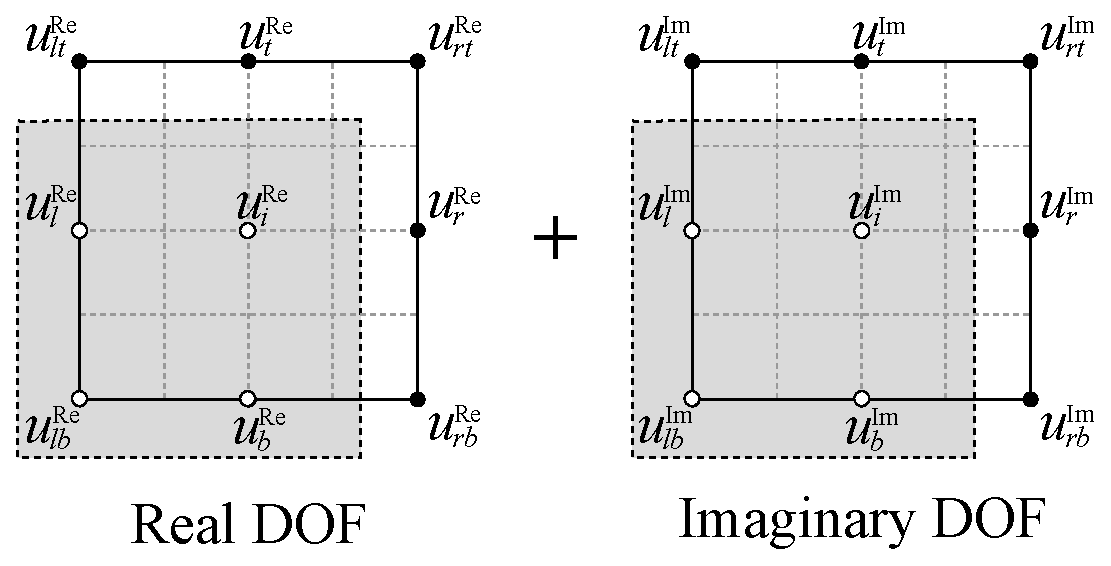
\includegraphics[height=6cm]{img/cell_FEM-real_algebra.pdf} 
\caption{Mesh for the real algebra implementation.}
\label{fig:double_mesh_real}
\end{figure}

We can express the values in boundary as
\begin{align*}
u_r(x_s) &= u_r^\text{Re}(x_s) + i u_r^\text{Im}(x_s)\\
t_r(x_s) &= t_r^\text{Re}(x_s) + i t_r^\text{Im}(x_s) \enspace ,
\end{align*}
and replacing these in \eqref{eq:bloch_cond}, we obtain
\begin{subequations}
\begin{align}
u_r^\text{Re}(x_s) &= u_r^\text{Re}(x_s + a_s)\cos(k_s a_s) + u_r^\text{Im}(x_s + a_s)\sin(k_s a_s)\\
u_r^\text{Im}(x_s) &= u_r^\text{Im}(x_s + a_s)\cos(k_s a_s) - u_r^\text{Re}(x_s + a_s)\sin(k_s a_s) \enspace ,
\end{align}
\label{eq:real_bloch_disp}
\end{subequations}
and
\begin{subequations}
\begin{align}
t_r^\text{Re}(x_s + a_s) &= -t_r^\text{Re}(x_s)\cos(k_s a_s) + t_r^\text{Im}(x_s)\sin(k_s a_s)\\
t_r^\text{Im}(x_s + a_s) &= -t_r^\text{Im}(x_s)\cos(k_s a_s) - t_r^\text{Re}(x_s)\sin(k_s a_s) \enspace .
\end{align}
\label{eq:real_bloch_trac}
\end{subequations}

In this case, the displacements and forces are arranged in block vectors as
\begin{align*}
\mathbf{U} &= \left[\mathbf{U}^\text{Re}\ \mathbf{U}^\text{Im}\right]^T\\
\mathbf{F} &= \left[\mathbf{F}^\text{Re}\ \mathbf{F}^\text{Im}\right]^T \ ,
\end{align*}
with
\begin{align*}
\mathbf{U}^\text{Re} &= \left[\mathbf{u}^\text{Re}_l\ \mathbf{u}^\text{Re}_r\ \mathbf{u}^\text{Re}_b\ \mathbf{u}^\text{Re}_t\ \mathbf{u}^\text{Re}_{lb}\ \mathbf{u}^\text{Re}_{rb}\ \mathbf{u}^\text{Re}_{lt}\ \mathbf{u}^\text{Re}_{rt}\ \mathbf{u}^\text{Re}_{i}\right]^T\\
\mathbf{U}^\text{Im} &=\left[\mathbf{u}^\text{Im}_l\ \mathbf{u}^\text{Im}_r\ \mathbf{u}^\text{Im}_b\ \mathbf{u}^\text{Im}_t\ \mathbf{u}^\text{Im}_{lb}\ \mathbf{u}^\text{Im}_{rb}\ \mathbf{u}^\text{Im}_{lt}\ \mathbf{u}^\text{Im}_{rt}\ \mathbf{u}^\text{Im}_{i}\right]^T \\
%%-- Forces
\mathbf{F}^\text{Re} &= \left[\mathbf{f}^\text{Re}_l\ \mathbf{f}^\text{Re}_r\ \mathbf{f}^\text{Re}_b\ \mathbf{f}^\text{Re}_t\ \mathbf{f}^\text{Re}_{lb}\ \mathbf{f}^\text{Re}_{rb}\ \mathbf{f}^\text{Re}_{lt}\ \mathbf{f}^\text{Re}_{rt}\ \mathbf{f}^\text{Re}_{i}\right]^T\\
\mathbf{F}^\text{Im} &= \left[\mathbf{f}^\text{Im}_l\ \mathbf{f}^\text{Im}_r\ \mathbf{f}^\text{Im}_b\ \mathbf{f}^\text{Im}_t\ \mathbf{f}^\text{Im}_{lb}\ \mathbf{f}^\text{Im}_{rb}\ \mathbf{f}^\text{Im}_{lt}\ \mathbf{f}^\text{Im}_{rt}\ \mathbf{f}^\text{Im}_{i}\right]^T \ .
\end{align*}

For the two dimensional example presented above the equations read
\begin{align*}
% u_r
\mathbf{u}^\text{Re}_r &= \mathbf{u}^\text{Re}_l\cos(\psi_x) - \mathbf{u}^\text{Im}_l\sin(\psi_x)\\
\mathbf{u}^\text{Im}_r &= \mathbf{u}^\text{Im}_l\cos(\psi_x) + \mathbf{u}^\text{Re}_l\sin(\psi_x)\\
% u_t
\mathbf{u}^\text{Re}_t &= \mathbf{u}^\text{Re}_b\cos(\psi_y) - \mathbf{u}^\text{Im}_b\sin(\psi_y)\\
\mathbf{u}^\text{Im}_t &= \mathbf{u}^\text{Im}_b\cos(\psi_y) + \mathbf{u}^\text{Re}_b\sin(\psi_y)\\
% u_{rb}
\mathbf{u}^\text{Re}_{rb} &= \mathbf{u}^\text{Re}_{lb}\cos(\psi_x) - \mathbf{u}^\text{Im}_{lb}\sin(\psi_x)\\
\mathbf{u}^\text{Im}_{rb} &= \mathbf{u}^\text{Im}_{lb}\cos(\psi_x) + \mathbf{u}^\text{Re}_{lb}\sin(\psi_x)\\
% u_{lt}
\mathbf{u}^\text{Re}_{lt} &= \mathbf{u}^\text{Re}_{lb}\cos(\psi_y) - \mathbf{u}^\text{Im}_{lb}\sin(\psi_y)\\
\mathbf{u}^\text{Im}_{lt} &= \mathbf{u}^\text{Im}_{lb}\cos(\psi_y) + \mathbf{u}^\text{Re}_{lb}\sin(\psi_y)\\
% u_{rt}
\mathbf{u}^\text{Re}_{rt} &= \mathbf{u}^\text{Re}_{lb}\cos(\psi_x + \psi_y) - \mathbf{u}^\text{Im}_{lb}\sin(\psi_x + \psi_y)\\
\mathbf{u}^\text{Im}_{rt} &= \mathbf{u}^\text{Im}_{lb}\cos(\psi_x + \psi_y) + \mathbf{u}^\text{Re}_{lb}\sin(\psi_x + \psi_y) \enspace ,
\end{align*}
where $\psi_x$ and $\psi_y$ are the phase shifts in $x$ and $y$. Similar expressions hold for the forces. Although the expressions are written explicitly here, they are all contained compactly in \eqref{eq:real_bloch_disp} and \eqref{eq:real_bloch_trac}. The phase shift is $\psi = k_j d_j$, with $k_j$ the components of the wave vector and $d_j$ the distance between the image and reference node in $j$ direction.

\begin{algorithm}[h]  
\DontPrintSemicolon
\SetKwInOut{Input}{Input}\SetKwInOut{Output}{Output}
\Input{ $k_x$, $k_y$, $k_z$: wave-vector components\\
		nodes: array with nodal coordinates\\
		image, reference: array with corresponding image and reference nodes
}
\Output{List of Multipoint constraints}
\BlankLine
ncond $\leftarrow$ Size of image\;
\For(){ i=1 \KwTo ncond}{
	x\_img, y\_img, z\_img $\leftarrow$ coordinates of image[i]\;
	x\_ref, y\_ref, z\_ref $\leftarrow$ coordinates of reference[i]\;
	$\psi$ $\leftarrow$ $k_x$(x\_img - x\_ref) + $k_y$(y\_img - y\_ref) + $k_z$(z\_img - z\_ref)\;
	$u_\text{img}^\text{Re}\ \leftarrow\ u_\text{ref}^\text{Re}\cos\psi + u_\text{ref}^\text{Im}\sin\psi$\;
	$u_\text{img}^\text{Im}\ \leftarrow\ u_\text{ref}^\text{Im}\cos\psi - u_\text{ref}^\text{Re}\sin\psi$\;
}

\caption{Generate the list of Multipoint constraints for the Bloch-periodic imposition using real algebra.}\label{algo:bloch_MPC_real}
\end{algorithm}